%%%%%%%%%%%%%%%%%%%%%%%%%%%%%%%%%%%%%%%%%
% Beamer Presentation
% LaTeX Template
% Version 1.0 (10/11/12)
%
% This template has been downloaded from:
% http://www.LaTeXTemplates.com
%
% License:
% CC BY-NC-SA 3.0 (http://creativecommons.org/licenses/by-nc-sa/3.0/)
%
%%%%%%%%%%%%%%%%%%%%%%%%%%%%%%%%%%%%%%%%%

%----------------------------------------------------------------------------------------
%	PACKAGES AND THEMES
%----------------------------------------------------------------------------------------

\documentclass{beamer}

\mode<presentation> {

  % The Beamer class comes with a number of default slide themes
  % which change the colors and layouts of slides. Below this is a list
  % of all the themes, uncomment each in turn to see what they look like.

  %\usetheme{default}
  %\usetheme{AnnArbor}
  %\usetheme{Antibes}
  %\usetheme{Bergen}
  \usetheme{Berkeley}
  %\usetheme{Berlin}
  %\usetheme{Boadilla}
  %\usetheme{CambridgeUS}
  %\usetheme{Copenhagen}
  %\usetheme{Darmstadt}
  %\usetheme{Dresden}
  %\usetheme{Frankfurt}
  %\usetheme{Goettingen}
  %\usetheme{Hannover}
  %\usetheme{Ilmenau}
  %\usetheme{JuanLesPins}
  %\usetheme{Luebeck}
  %\usetheme{Madrid}
  %\usetheme{Malmoe}
  %\usetheme{Marburg}
  %\usetheme{Montpellier}
  %\usetheme{PaloAlto}
  %\usetheme{Pittsburgh}
  %\usetheme{Rochester}
  %\usetheme{Singapore}
  %\usetheme{Szeged}
  %\usetheme{Warsaw}

  % As well as themes, the Beamer class has a number of color themes
  % for any slide theme. Uncomment each of these in turn to see how it
  % changes the colors of your current slide theme.

  %\usecolortheme{albatross}
  %\usecolortheme{beaver}
  %\usecolortheme{beetle}
  %\usecolortheme{crane}
  %\usecolortheme{dolphin}
  %\usecolortheme{dove}
  %\usecolortheme{fly}
  %\usecolortheme{lily}
  %\usecolortheme{orchid}
  %\usecolortheme{rose}
  %\usecolortheme{seagull}
  %\usecolortheme{seahorse}
  %\usecolortheme{whale}
  %\usecolortheme{wolverine}

  %\setbeamertemplate{footline} % To remove the footer line in all slides uncomment this line
  %\setbeamertemplate{footline}[page number] % To replace the footer line in all slides with a simple slide count uncomment this line

  %\setbeamertemplate{navigation symbols}{} % To remove the navigation symbols from the bottom of all slides uncomment this line
}

\usepackage{graphicx} % Allows including images
\usepackage{booktabs} % Allows the use of \toprule, \midrule and \bottomrule in tables

%----------------------------------------------------------------------------------------
%	TITLE PAGE
%----------------------------------------------------------------------------------------

\title[GL Transformations]{Matrices, GL Transformations} % The short title appears at the bottom of every slide, the full title is only on the title page

\author{Dane Christensen, Brigham H. Keys, Esq.} % Your name
\institute[BYU-Idaho] % Your institution as it will appear on the bottom of every slide, may be shorthand to save space
          {
            Brigham Young University - Idaho\\
            \medskip
            \textit{key13005@byui.edu} % Your email address
          }
          \date{\today} % Date, can be changed to a custom date

          \begin{document}

          \begin{frame}
            \titlepage % Print the title page as the first slide
            
\includegraphics[scale=.1]{../logo.png}
          \end{frame}

          %----------------------------------------------------------------------------------------
          %	PRESENTATION SLIDES
          %----------------------------------------------------------------------------------------

          \section{Matrices} % A subsection can be created just before a set of slides with a common theme to further break down your presentation into chunks

          \begin{frame}
            \frametitle{Matrices}
            Matrix math is the building block of everything OpenGL does. Matrices add a W to our X, and Y coordinate system. W will specify whether or not it is a point in space, or a direction. Much like functions, matrices are in a stack in OpenGL and can be ``pushed'' or ``popped''.
          \end{frame}

          %-------------------------------------------------
          \subsection{Push and Pop}
          \begin{frame}
            \frametitle{Push and Pop Matrices}
            There are at least 2 matrices on our OpenGL stack at any given moment. However whenever we use 3D graphics there will be at least 32 matrices. We can push and pop these matrices just like we can functions on a stack.\\
            \begin{block}{glPopMatrix(void);}
              Pops the current matrix, replacing the matrix below it.\\
            \end{block}

            \begin{block}{glPushMatrix(voidX);}
              Pushes the current matrix, adding a matrix above it.\\
            \end{block}
          \end{frame}

          \section{Transform in OpenGL}

          %------------------------------------------------

          \subsection{glRotate}
          \begin{frame}
            \frametitle{glRotate}
            glRotate rotates by angle around our shape. The function generates a rotation matrix, that is multiplied by our current matrix. The product of this multiplication replaces our current matrix.
            \begin{block}{void glRotatef(GLfloat angle,  GLfloat x,  GLfloat y,  GLfloat z);}
              \begin{itemize}
              \item angle -- specifies in degrees how far to rotate the matrix.
              \item x, y, z -- The angles to be rotated. simply pass 0 in if you wish to not rotate by that dimension simply pass 0.0 as the parameter.
              \end{itemize}
            \end{block}
            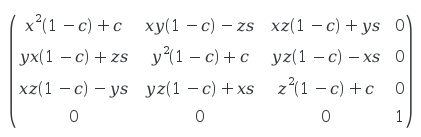
\includegraphics[scale=.35]{rotate_matrix.png}
          \end{frame}


          %-------------------------------------------------

          %------------------------------------------------

          \subsection{glScale}
          \begin{frame}
            \frametitle{glScale}
            glScale will scale differently to each axis, unless the scale factor for x, y, and z are all equal. Each parameter represents the scale to factor each axis
            \begin{block}{void glScalef(GLfloat x, GLfloat y, GLfloat z);}
              \begin{itemize}
              \item x, y, z -- factor of how each axis should be scaled.
              \end{itemize}
            \end{block}
            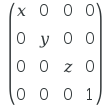
\includegraphics[scale=.35]{scale_matrix.png}
          \end{frame}

          %------------------------------------------------

          \subsection{glScale}
          \begin{frame}
            \frametitle{glTranslate}
            glTranslate produces a translation matrix that is multiplied by our current matrix. Our current matrix is replaced by the product.
            \begin{block}{void glTranslated(GLdouble x, GLdouble y, GLdouble z);}
              \begin{itemize}
              \item x, y, z -- factor of how each axis should be translated.
              \end{itemize}
            \end{block}
            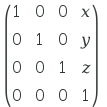
\includegraphics[scale=.35]{translate_matrix.png}
          \end{frame}


          %------------------------------------------------
          \section{Second Section}
          %------------------------------------------------
          \begin{frame}
            \frametitle{glList}
            Lists in OpenGL allow us to compile code at runtime, and assign a tag to the code that was compiled. Useful when maximizing information hiding when using classes.
          \end{frame}
          %-------------END SLIDE--------------------------

          %-------------BEGIN SLIDE------------------------
          \begin{frame}
            \frametitle{References}
            \footnotesize {
              \begin{thebibliography}{99}
              \bibitem[OpenGL, 2015]{p1} https://www.opengl.org/ (2015)
              \end{thebibliography}
            }
            
\includegraphics[scale=.33]{../cc.png}

          \end{frame}
          %-------------END SLIDE--------------------------

          \end{document} 
